\documentclass[12pt]{article}
\usepackage{bbm}
\usepackage{fancyhdr}
\usepackage{titling}
\usepackage{enumitem}
\usepackage{amsmath}
\usepackage{dsfont}
\usepackage{amsfonts}
\usepackage{amssymb}
\usepackage{amsthm}
\usepackage{geometry}
\usepackage{tikz}
\usepackage{algorithm}
\usepackage{algpseudocode}
\geometry{verbose,tmargin=1in,bmargin=1in,lmargin=1in,rmargin=1in}
\renewcommand{\vec}[1]{\mathbf{#1}}
\newcommand{\dec}{\text{dec}}
\newcommand{\divi}{\mathbin{\textnormal{div}}}
\title{Homework 1}
\author{Satvik Prasad}
\date{}
\newtheorem{lemma}{Lemma}[section]
\fancypagestyle{plain}{%
  \fancyhf{}
  \fancyhead[L]{\theauthor}
  \fancyhead[R]{\thedate}
}
\pagestyle{plain}
\makeatletter
\def\@maketitle{%
  \newpage
  \null
  \vskip 1em%
  \begin{center}%
    \let \footnote \thanks
    {\LARGE \@title \par}%
    \vskip 1em%
  \end{center}%
  \par
\vskip 1em}
\makeatother
\usepackage{cmbright}

\newcommand{\mat}[1]{\mathbf{#1}}

% ---------- Probability theory ----------
% Core operators (optional argument-free; use as \E{X}, \Var{X}, \Cov{X}{Y})
\DeclareMathOperator{\EOp}{\mathbb{E}}
\DeclareMathOperator{\VarOp}{Var}
\DeclareMathOperator{\CovOp}{Cov}
\DeclareMathOperator{\CorrOp}{Corr}

\renewcommand{\P}[1]{\mathbb{P}\left(#1\right)}        % \P{A}
\newcommand{\E}[1]{\EOp\left[#1\right]}                % \E{X}
\newcommand{\Var}[1]{\VarOp\left(#1\right)}            % \Var{X}
\newcommand{\Cov}[2]{\CovOp\left(#1,\,#2\right)}       % \Cov{X}{Y}
\newcommand{\Corr}[2]{\CorrOp\left(#1,\,#2\right)}     % \Corr{X}{Y}
\newcommand{\SD}[1]{\operatorname{SD}\left(#1\right)}  % \SD{X}

% Subscripted versions, e.g. \Esub{\theta}{X}, \Psub{\theta}{A}
\newcommand{\Esub}[2]{\EOp_{#1}\left[#2\right]}
\newcommand{\Psub}[2]{\mathbb{P}_{#1}\left(#2\right)}

% Conditioning, indicators, independence
\newcommand{\given}{\,\middle|\,}                      % \E{X \given Y}
\newcommand{\ind}[1]{\mathbbm{1}\left\{#1\right\}}     % \ind{X > 0}
\newcommand{\indep}{\perp\!\!\!\perp}                  % X \indep Y
\newcommand{\iid}{\overset{\text{iid}}{\sim}}          % X_i \iid \Normal(0,1)

% Convergence
\newcommand{\convp}{\xrightarrow{\;p\;}}               % in probability
\newcommand{\convd}{\xrightarrow{\;d\;}}               % in distribution
\newcommand{\convas}{\xrightarrow{\text{a.s.}}}        % almost surely
\newcommand{\convLp}[1]{\xrightarrow{L^{#1}}}          % in L^p

% Probability spaces
\newcommand{\F}{\mathcal{F}}                           % sigma-algebra
\newcommand{\B}{\mathcal{B}}                           % Borel sigma-algebra
\newcommand{\pspace}{(\Omega, \F, \mathbb{P})}

% Common distributions
\newcommand{\Normal}{\mathcal{N}}
\newcommand{\Bern}{\operatorname{Bernoulli}}
\newcommand{\Bin}{\operatorname{Binomial}}
\newcommand{\Pois}{\operatorname{Poisson}}
\newcommand{\Unif}{\operatorname{Uniform}}
\newcommand{\Exp}{\operatorname{Exp}}
\newcommand{\Geom}{\operatorname{Geometric}}
\newcommand{\Gam}{\operatorname{Gamma}}
\newcommand{\Beta}{\operatorname{Beta}}

% Number sets
\newcommand{\R}{\mathbb{R}}
\newcommand{\N}{\mathbb{N}}
\newcommand{\Z}{\mathbb{Z}}


\begin{document}
\subsection{Writing Proofs}
\begin{enumerate}
  \item Assume we have such a subspace $U,$ with some non-zero
    element $u \in U,$ and some element $v \not \in U, $ with $v \in
    V.$ Then, we can always construct some map $T$ with $Tu = v,$
    meaning there's some map where $U$ is not invariant. Hence,
    either there is no such $u$, or no such $v.$

    If there is no such $u,$ then $U = \{0\}.$ Alternatively, if
    there is no such $v,$ we have $U = V$ as required.

  \item For $v \in V$  to be an eigenvalue of $P,$ we have $Pv =
    \lambda v$ for some $\lambda \in \mathbb F,$ and $v \neq 0.$
    Since $U \oplus W  = V$ is a direct sum, there are some unique
    $u, w$ with $u + w = v,$ and $u \in U,$ $w \in W.$

    Therefore, we have $$
    u = \lambda(u + w) \Rightarrow (\lambda - 1)u + \lambda w = 0.
    $$
    By the properties of the direct sum, this is only the case when
    $(\lambda - 1)u = 0$ or $\lambda w = 0.$ Hence, we have cases:
    \begin{itemize}
      \item If $u = 0,$ then $w \neq 0,$ meaning $\lambda = 0$ and $w
        \in W \setminus\{0\}$ is free.
      \item If $\lambda = 1,$ then $w = 0,$ meaning $u \in U
        \setminus \{0\}$ is free.
    \end{itemize}

    Thus, we have eigenvalues $0, 1$ with eigenvectors $w \in W$ and
    $u \in U$ respectively (excluding the trivial $0$ vector).

  \item
    \begin{itemize}
      \item Let us assume $T$ has an eigenvalue of $\lambda \in
        \mathbb F.$ Then, there exists some non-zero $v$ such that
        $Tv = \lambda v.$ Applying a left-inverse, we have
        $$
        v = \lambda T^{-1} v \Rightarrow T^{-1}v = \dfrac{1}{\lambda } v,
        $$
        meaning $T^{-1}$ has an eigenvalue of $\lambda^{-1}.$

        Conversely, if $T^{-1}$ has eigenvalue $1/\lambda,$ we know
        for some $v \neq 0$
        $$
        T^{-1} v = \dfrac{1}{\lambda}{v} \Rightarrow \lambda v = Tv,
        $$
        and hence $\lambda$ is an eigenvalue of $T$ as required.

      \item Assume $T$ has some eigenvector $v.$ Then by the above,
        $T^{-1}$ has eigenvector $v.$ By the above, the converse is
        also true. Hence, $T$ has eigenvector $v$ if and only if
        $T^{-1}$ has eigenvector $v,$ meaning $T, T^{-1}$ have the
        same eigenvectors.
    \end{itemize}

  \item Apply $T$ to some vector $v$ repeatedly until the list
    becomes linearly dependent. Hence, we have
    $$
    Iv = (w, z), \qquad Tv = (-z, w), \qquad T^2v = (-w, -z).
    $$
    For a linear combination to be $0,$ we need
    \begin{align*}
      (\lambda_1 -1)w - \lambda_2 z  &= 0, \\
      (\lambda_1 -1)z + \lambda_2 w  &= 0, \\
    \end{align*}
    for all $w, z.$ This is true for all $\lambda_1 = 1$ and
    $\lambda_2 = 0,$ meaning
    $$
    I + T^2 = 0,
    $$
    i.e., minimal polynomial is $p \in \mathcal P_2(\mathbb F)$ with
    $p(x) = 1+ x^2.$

  \item Suppose that we have finite dimensional $V,$ and some map $T
    \in \mathcal L(V),$ with minimal polynomial $p \in \mathcal
    P(\mathbb F).$ I.e.,
    $$
    p(T) v = 0
    $$
    for all $v \in V.$

    Then, let us look at $p(T') \varphi$ for some arbitrary $\varphi
    \in V'.$ Let us write $p(T')$ as
    $$
    p(T')\varphi = \left(\sum_{k = 0}^{m} a_k (T')^{k} \right) \varphi
    $$
    for $m = \deg p.$ Hence, we get
    $$
    p(T') \varphi = \sum_{k = 0}^{m} a_k (\varphi \circ T^{k} ) =
    \varphi \circ \left(
      \sum_{k = 0}^{m} a_k T^{k}
    \right) = \varphi \circ p(T) = \varphi \circ 0 = 0.
    $$
    Hence, $p$ is also a minimal polynomial for $T'.$ Since minimal
    polynomials are unique, $T$ and $T'$ have the same minimal polynomials.
\end{enumerate}

\subsection{Evaluating Proofs}
In the forward direction, we correctly derive that for some $v \neq
0,$ $(T'\varphi)(v) = \lambda \varphi(v).$ However, for $T' \varphi =
\lambda \varphi,$ we need this to hold for all $v.$ Thus, the forward
direction is insufficient.

Additionally, in the reverse direction we derive that for some
$\varphi \in V',$ any $v \in V$ satisfies $$
\varphi(\lambda v) = \varphi(Tv).
$$
However, $\varphi \in V'$ is not necessarily injective, meaning we
can't derive $Tv = \lambda v$ for some $v \neq 0,$ and hence our proof fails.'

\subsection{Using Computers}
\begin{center}
  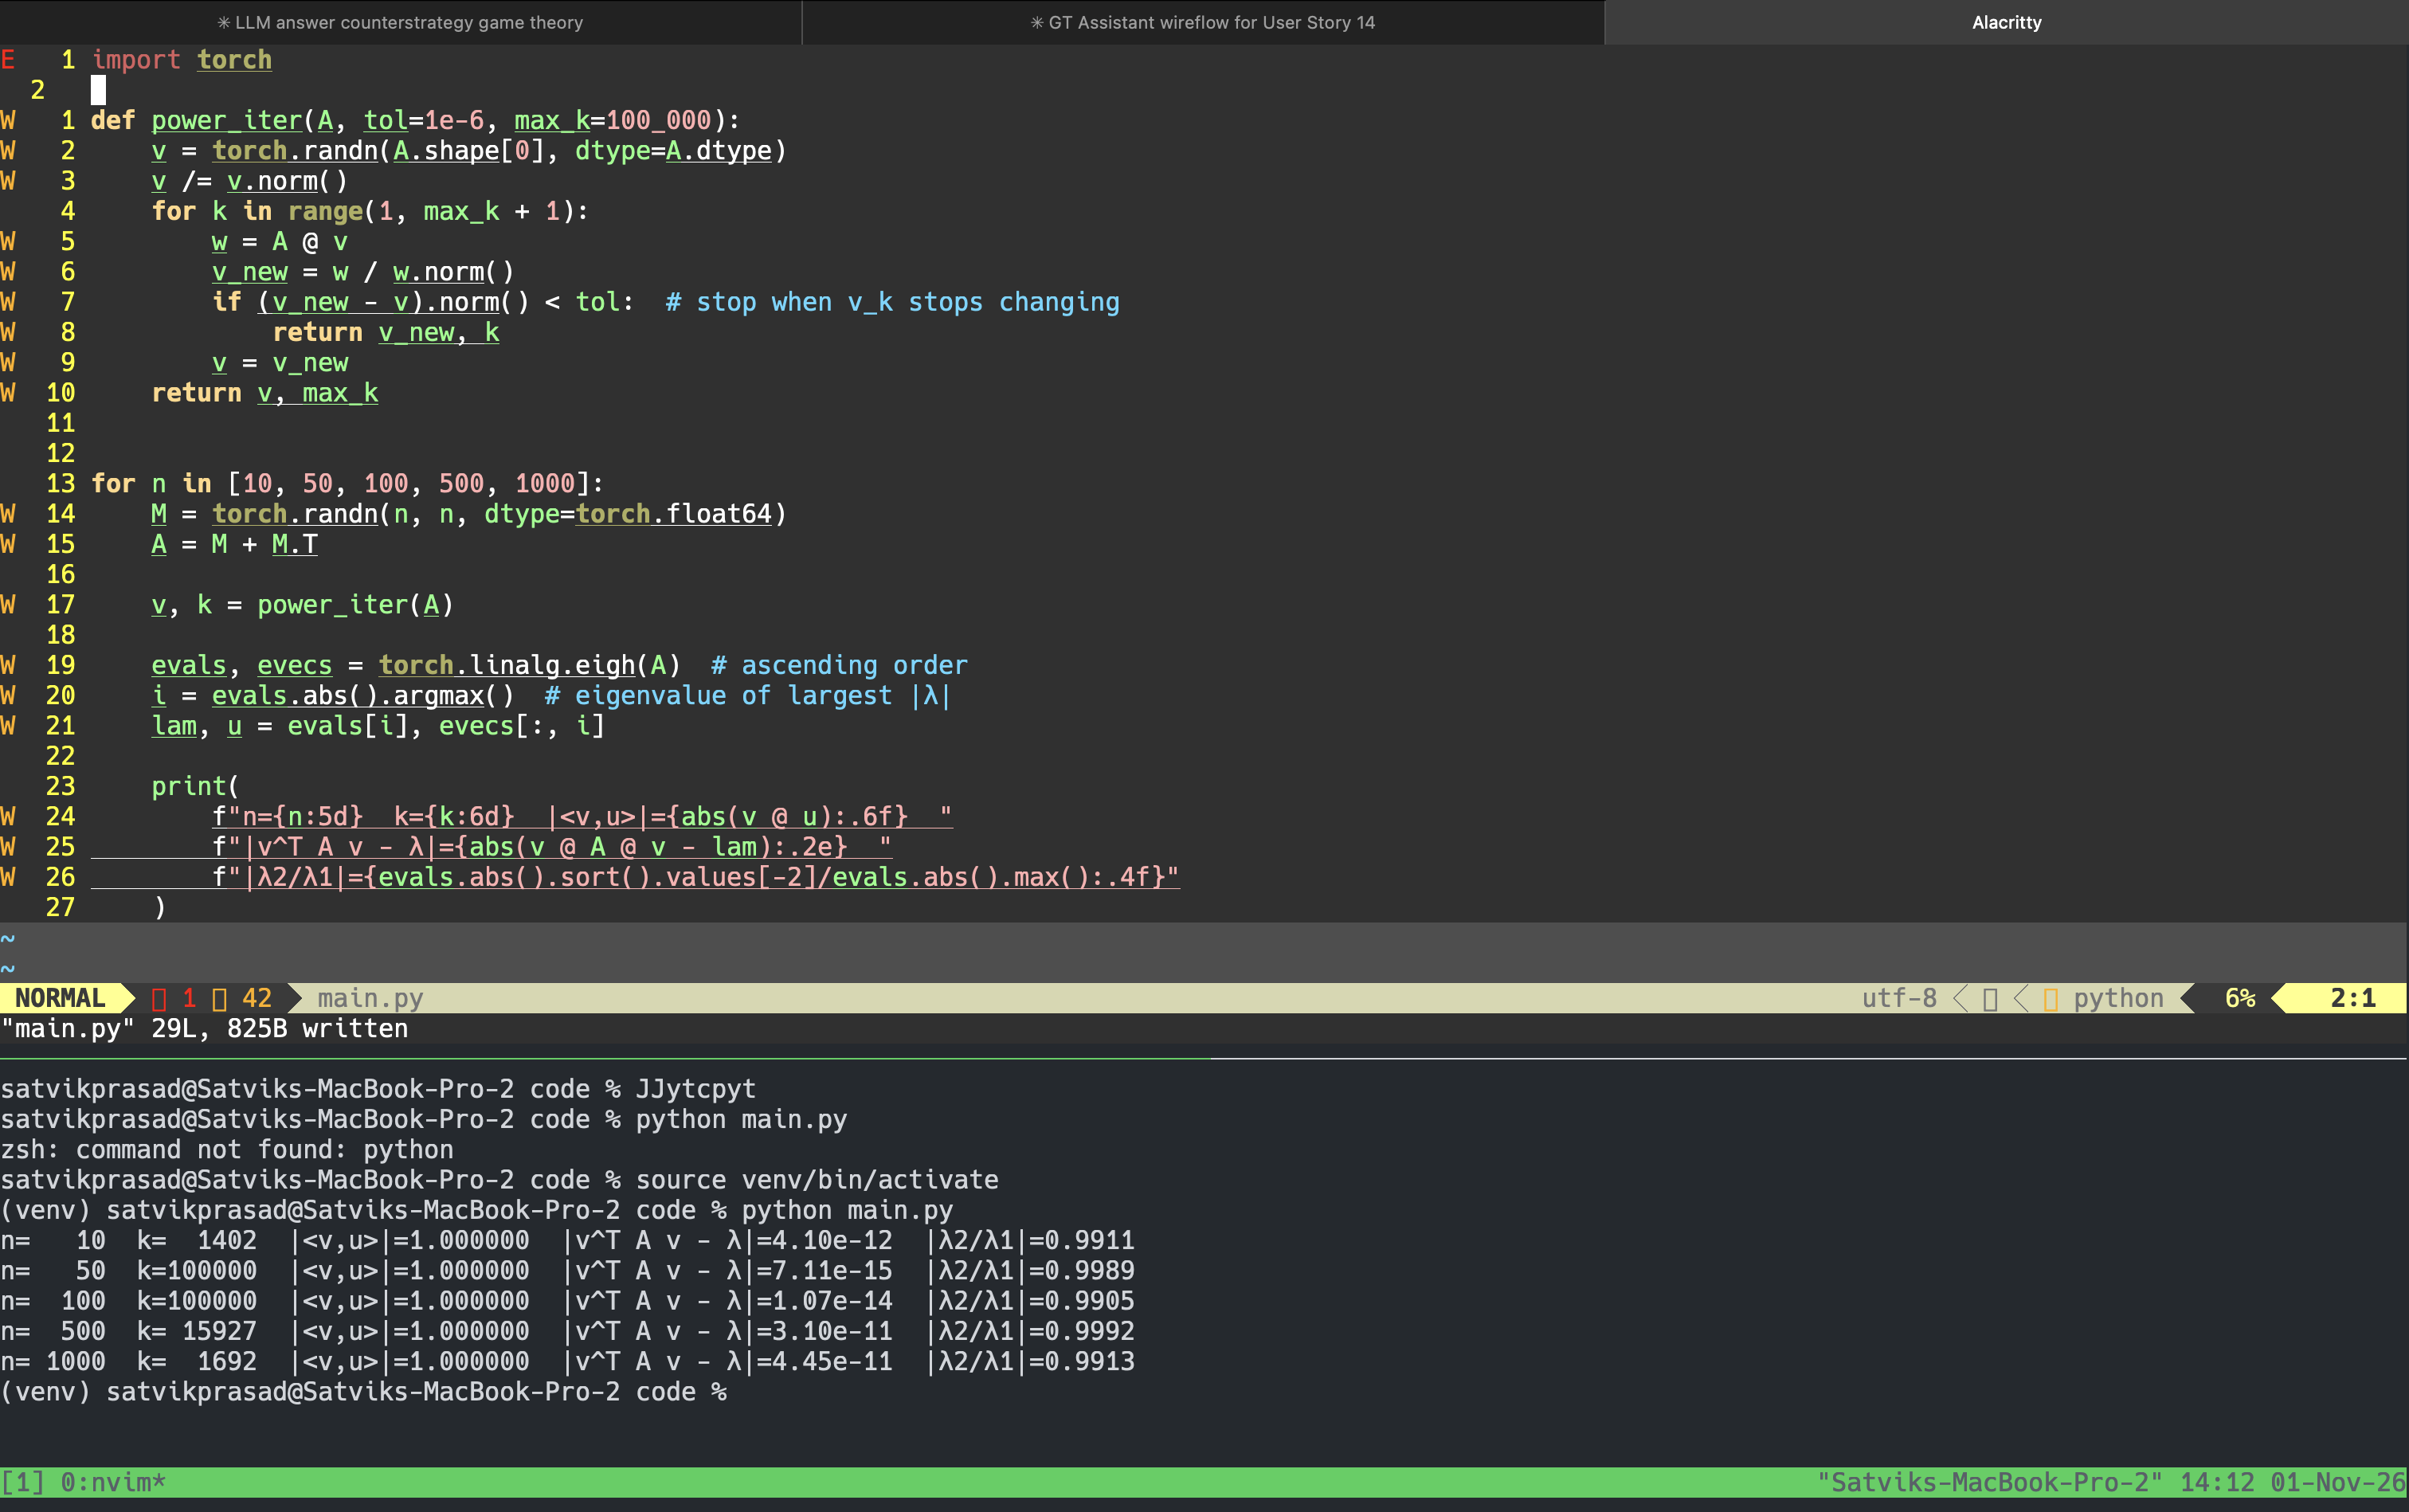
\includegraphics[width=0.9\linewidth]{math3406/blah.png}
\end{center}
Based on the code's output, the eigenvectors point in incredibly
similar directions, and the ratio of the magnitude of the eigenvalues
is very high too, suggesting the claim is correct.

\end{document}
